An object of this class represents a loop in the code of the application being
instrumented. We detect both natural loops (single-entry loops) and
irreducible loops
(multi-entry loops). For a natural loop, it has only one entry block
and this entry
block dominates all blocks in the loop; thus the entry block is also called the
head or the header of the loop. However, for an irreducible loop, it
has multiple
entry blocks and none of them dominates all blocks in the loop; thus there is no
head or header for an irreducible loop. The following figure
illustrates the difference:

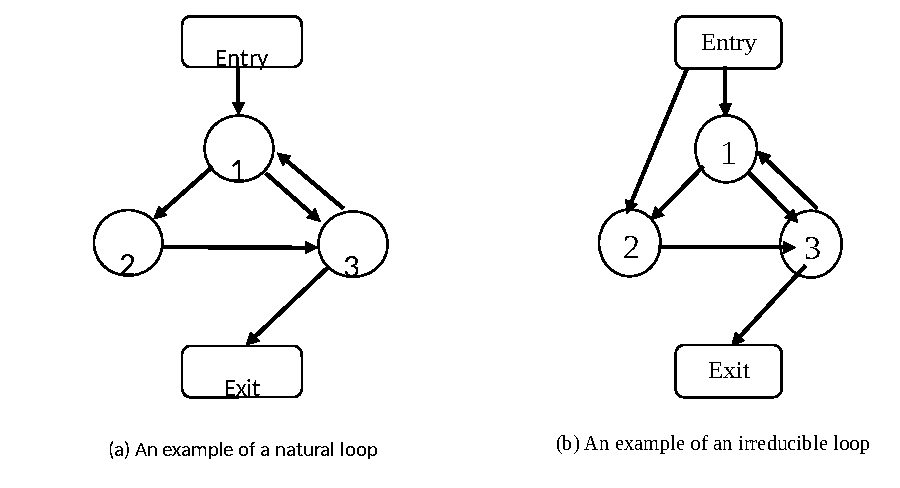
\includegraphics{loop_example}

Figure (a) above shows a natural loop, where block 1 represents the single entry
and block 1 is the head of the loop. Block 1 dominates block 2 and block 3.
Figure (b) above shows an irreducible loop, where block 1 and block 2
are the entries
of the loop. Neither block 1 nor block 2 domiantes block 3.

\begin{apient}
  bool containsAddress(unsigned long addr)
\end{apient}

\apidesc{
  Return true if addr is contained within any of the basic blocks that compose
  this loop, excluding the block of any of its sub-loops.
}
\begin{apient}
  bool containsAddressInclusive(unsigned long addr)
\end{apient}

\apidesc{
  Return true if addr is contained within any of the basic blocks that compose
  this loop, or in the blocks of any of its sub-loops.
}
\begin{apient}
  int getBackEdges(std::vector<BPatch_edge *> &edges)
\end{apient}

\apidesc{
  Returns the number of back edges in this loop and adds those edges
  to the edges vector. An edge is a back edge if it
  is from a block in the loop to an entry block of the loop.
}
\begin{apient}
  int getLoopEntries(std::vector<BPatch_basicBlock *> &entries)
\end{apient}

\apidesc{
  Returns the number of entry blocks of this loop and adds those
  blocks to the entries vector. An irreducible loop can
  have multiple entry blocks.
}
\begin{apient}
  bool getContainedLoops(std::vector<BPatch_basicBlockLoop*>&)
\end{apient}

\apidesc{
  Fill the given vector with a list of the loops nested within this loop.
}
\begin{apient}
  BPatch_flowGraph *getFlowGraph()
\end{apient}

\apidesc{
  Return a pointer to the control flow graph that contains this loop.
}
\begin{apient}
  bool getOuterLoops(std::vector<BPatch_basicBlockLoop*>&)
\end{apient}

\apidesc{
  Fill the given vector with a list of the outer loops nested within this loop.
}

\begin{apient}
  bool getLoopBasicBlocks(std::vector<BPatch_basicBlock*>&)
\end{apient}

\apidesc{
  Fill the given vector with a list of all basic blocks that are part
  of this loop.
}
\begin{apient}
  bool getLoopBasicBlocksExclusive(std::vector<BPatch_basicBlock*>&)
\end{apient}

\apidesc{
  Fill the given vector with a list of all basic blocks that are part
  of this loop but not its sub-loops.
}
\begin{apient}
  bool hasAncestor(BPatch_basicBlockLoop*)
\end{apient}

\apidesc{
  Return true if this loop is nested within the given loop (the given
  loop is one of its ancestors in the tree of loops).
}
\begin{apient}
  bool hasBlock(BPatch_basicBlock *b)
\end{apient}

\apidesc{
  Return true if this loop or any of its sub-loops contain b, false otherwise.
}
\begin{apient}
  bool hasBlockExclusive(BPatch_basicBlock *b)
\end{apient}

\apidesc{
  Return true if this loop, excluding its sub-loops, contains b,
  false otherwise.
}
